%UX diagrams
The purpose of the UX diagram is to show the different screens provided by the user interface of a particular application and their dynamic contents. Moreover it points out the interactions among the screens themselves and the presence of input forms and required data in a specific screen.

The diagrams provided below follow the User Interface requirements stated in the RASD document~\cite{rasd}.

The Web and the Mobile applications implement the same functionalities. This is why just a single UX diagram for both the applications has been attached to this document. Please notice that:
\begin{itemize}
\item \emph{\color{red} red} words describe functionalities accessible from the mobile application only (for example the provision of GPS data to the system);
\item the possible choices of the user (e.g.: the car to be rented, the GPS coordinates...) have been depicted as \emph{Input Forms} since they are data to be sent to the system and imply a screen update.
\end{itemize}
The UX diagram of the both the Web and Mobile applications is shown in Figure \ref{web_mobile_ux}. \\
The UX diagram of the on-board application is shown in Figure \ref{on_board_ux}.

\begin{figure}[H]
\begin{center}
		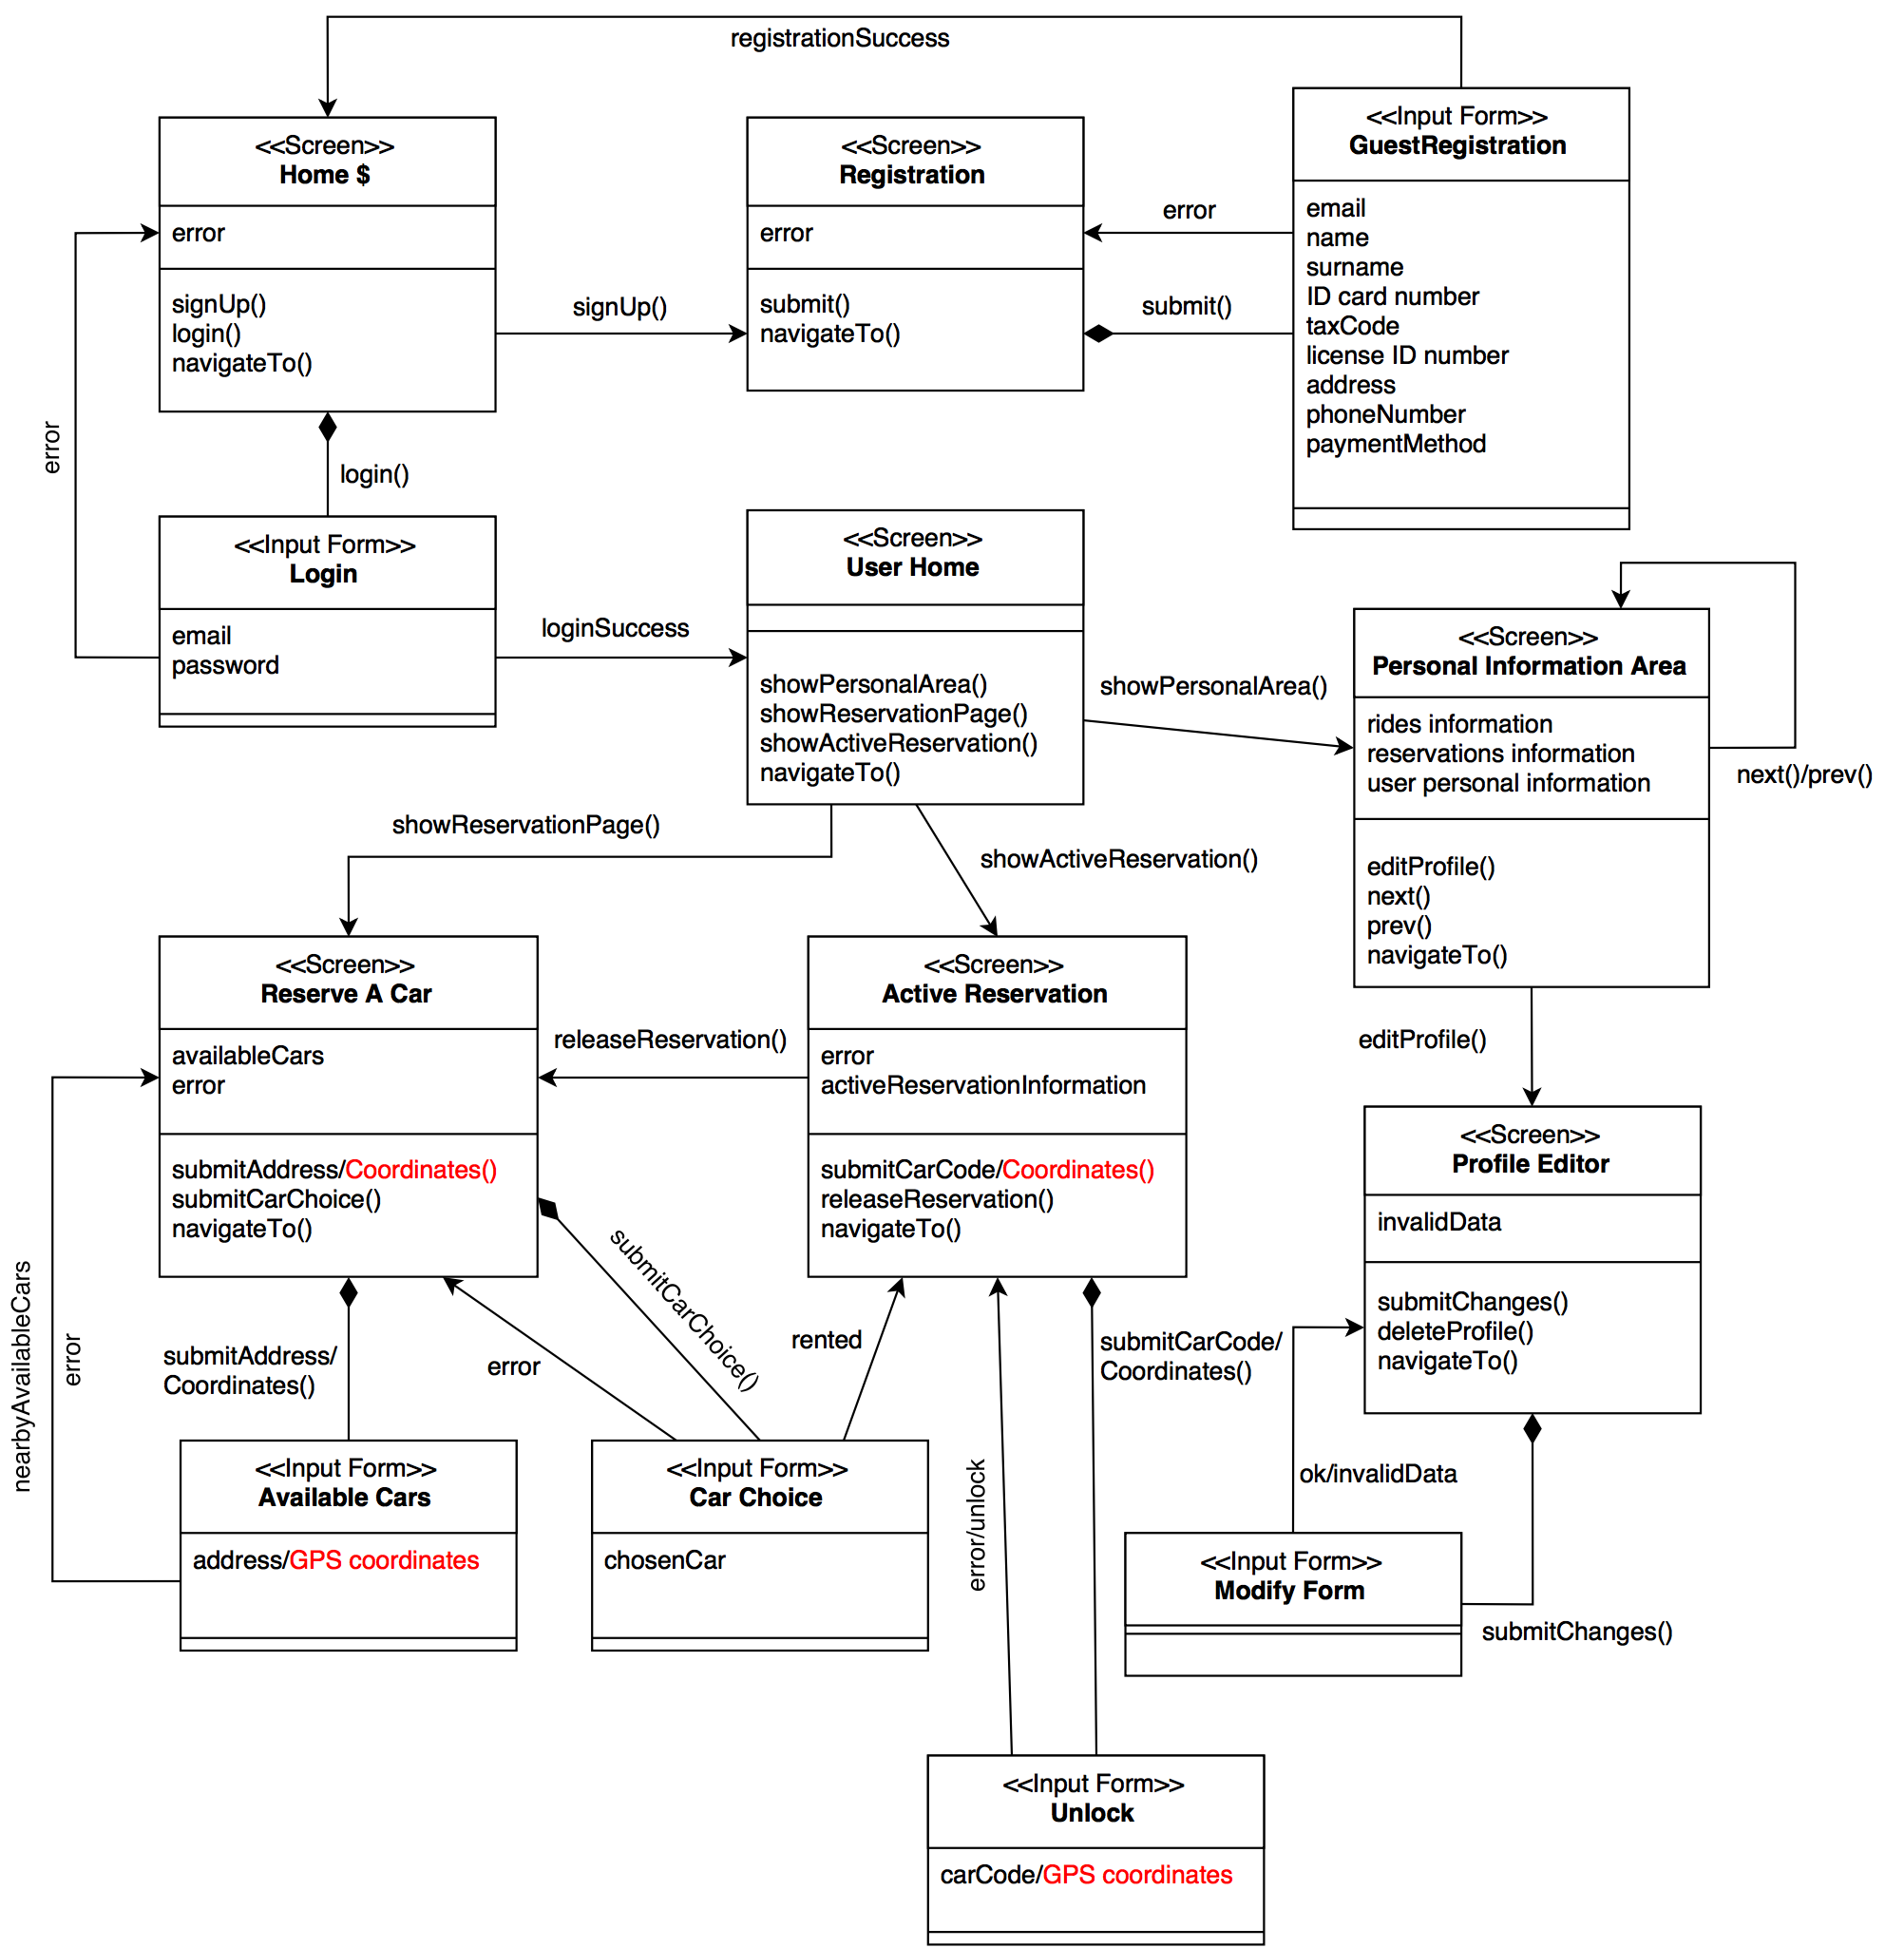
\includegraphics[width=\textwidth]{./user_interface_design/diagrams/web_mobile_ux.png}
		\caption{UX diagram of both the Web and the Mobile Applications. Note that the outgoing arcs exiting from "User Home" are mutually exclusive: they are shown based on the presence of an active reservation by the current user.}
		\label{web_mobile_ux}
\end{center}
\end{figure}

\begin{figure}[H]
\begin{center}
		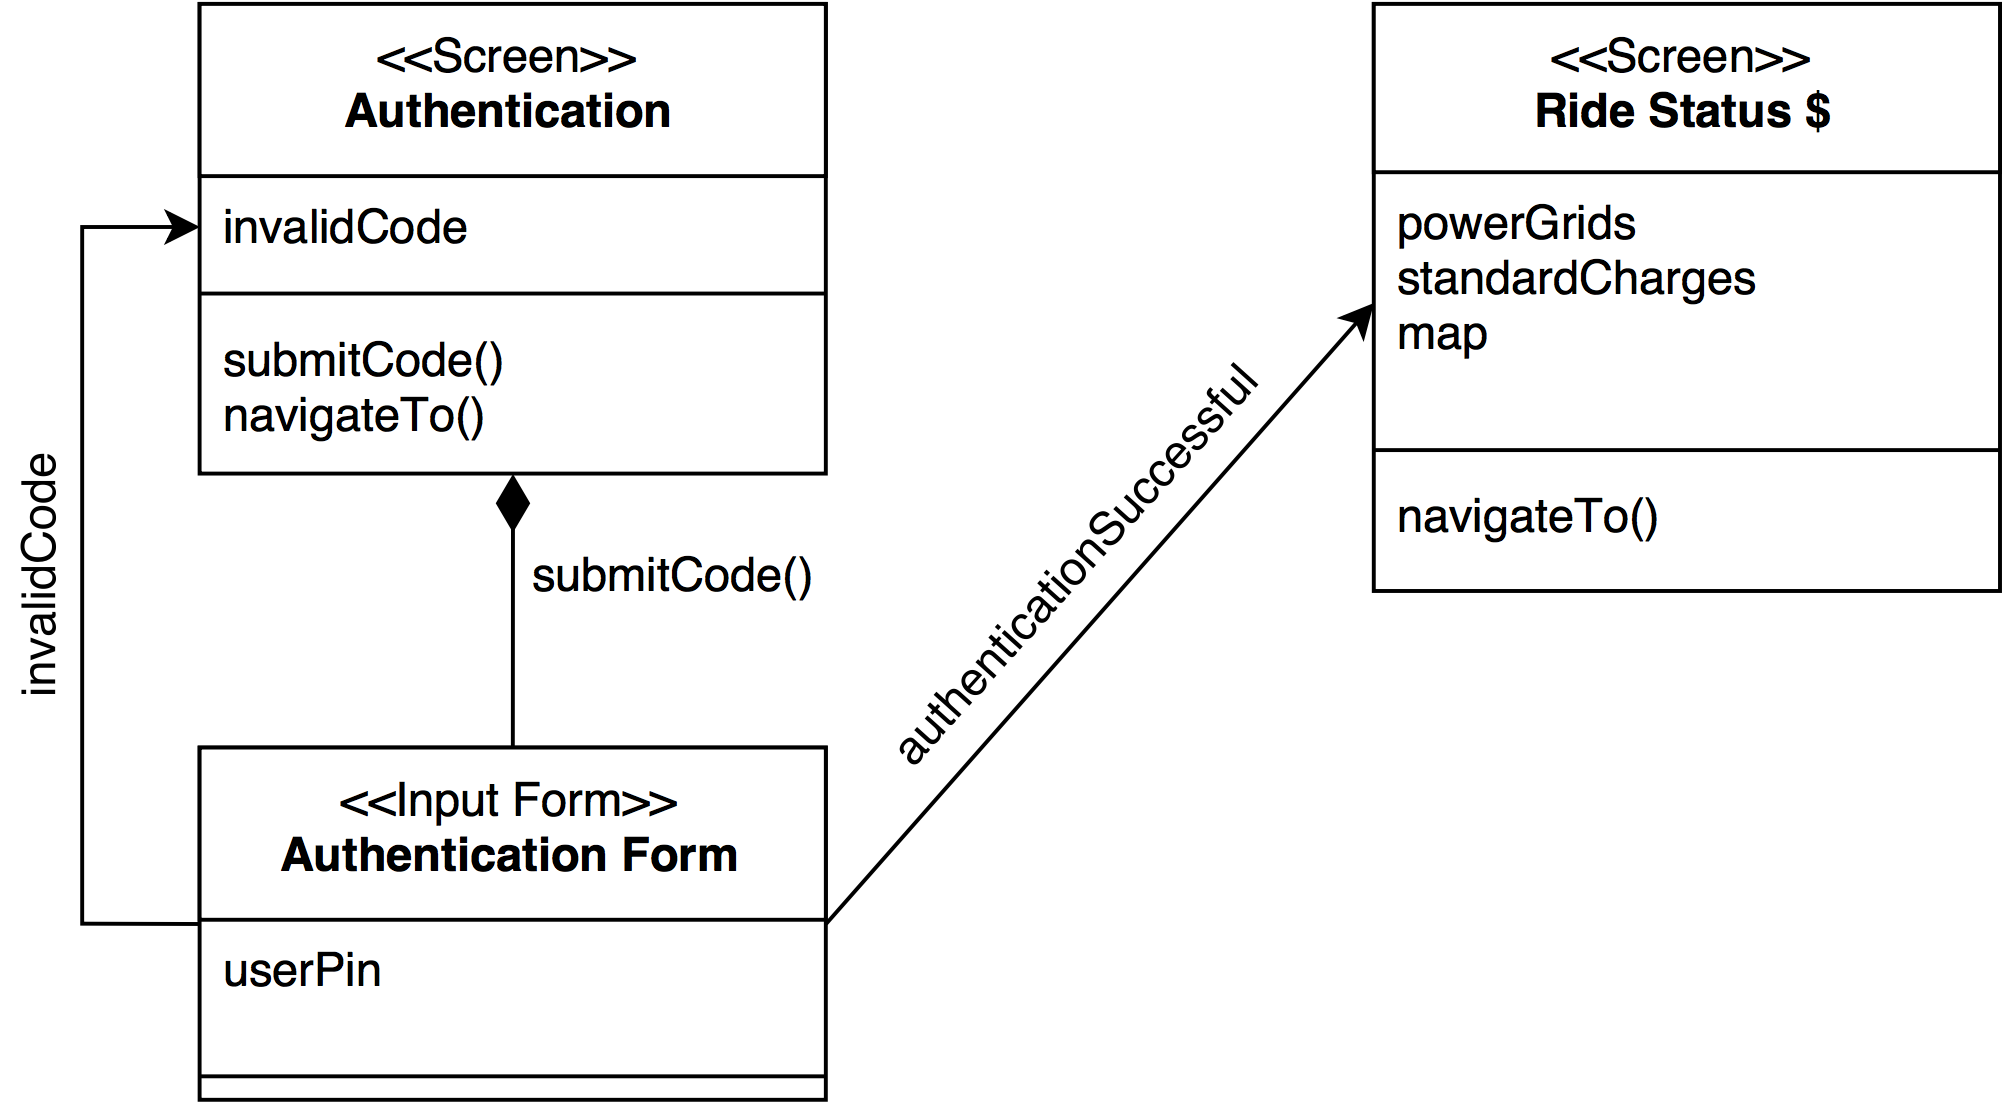
\includegraphics[width=\textwidth]{./user_interface_design/diagrams/on_board_ux.png}
		\caption{UX diagram of the On-Board Application. Notice that the attributes shown in the "Ride Status" screen are actually dynamic content. Note that there is no screen marked with the "\$" symbol: this is because no page acts as a home page reachable from anywhere in the application; the first screen to be shown is of course the "Authentication" one.}
		\label{on_board_ux}
\end{center}
\end{figure}